\chapter{Results}

The results for the model inspection and discuss the goodness of the fit model for the 2-lepton channel is shown in this section.

\section{Prefit plots}
Figure~\ref{fig:fit_2lep_prefit} shows the pre-fit plots of the analysis regions entering in the 2-lep only fit model. There are 3 SRs and Z+jets CRs;
in particular, \mjjtag distributions in \Zjets CRs are shown and the RNN scores distributions are shown in the SRs, only the left side bins are plotted using real data as well. The MC normalization shows a discrepancy compared to data, while the slope observed in Chapter is corrected with the reweighting, which is to be fitted in the final fitting.

\begin{figure}[ht]
    \centering
    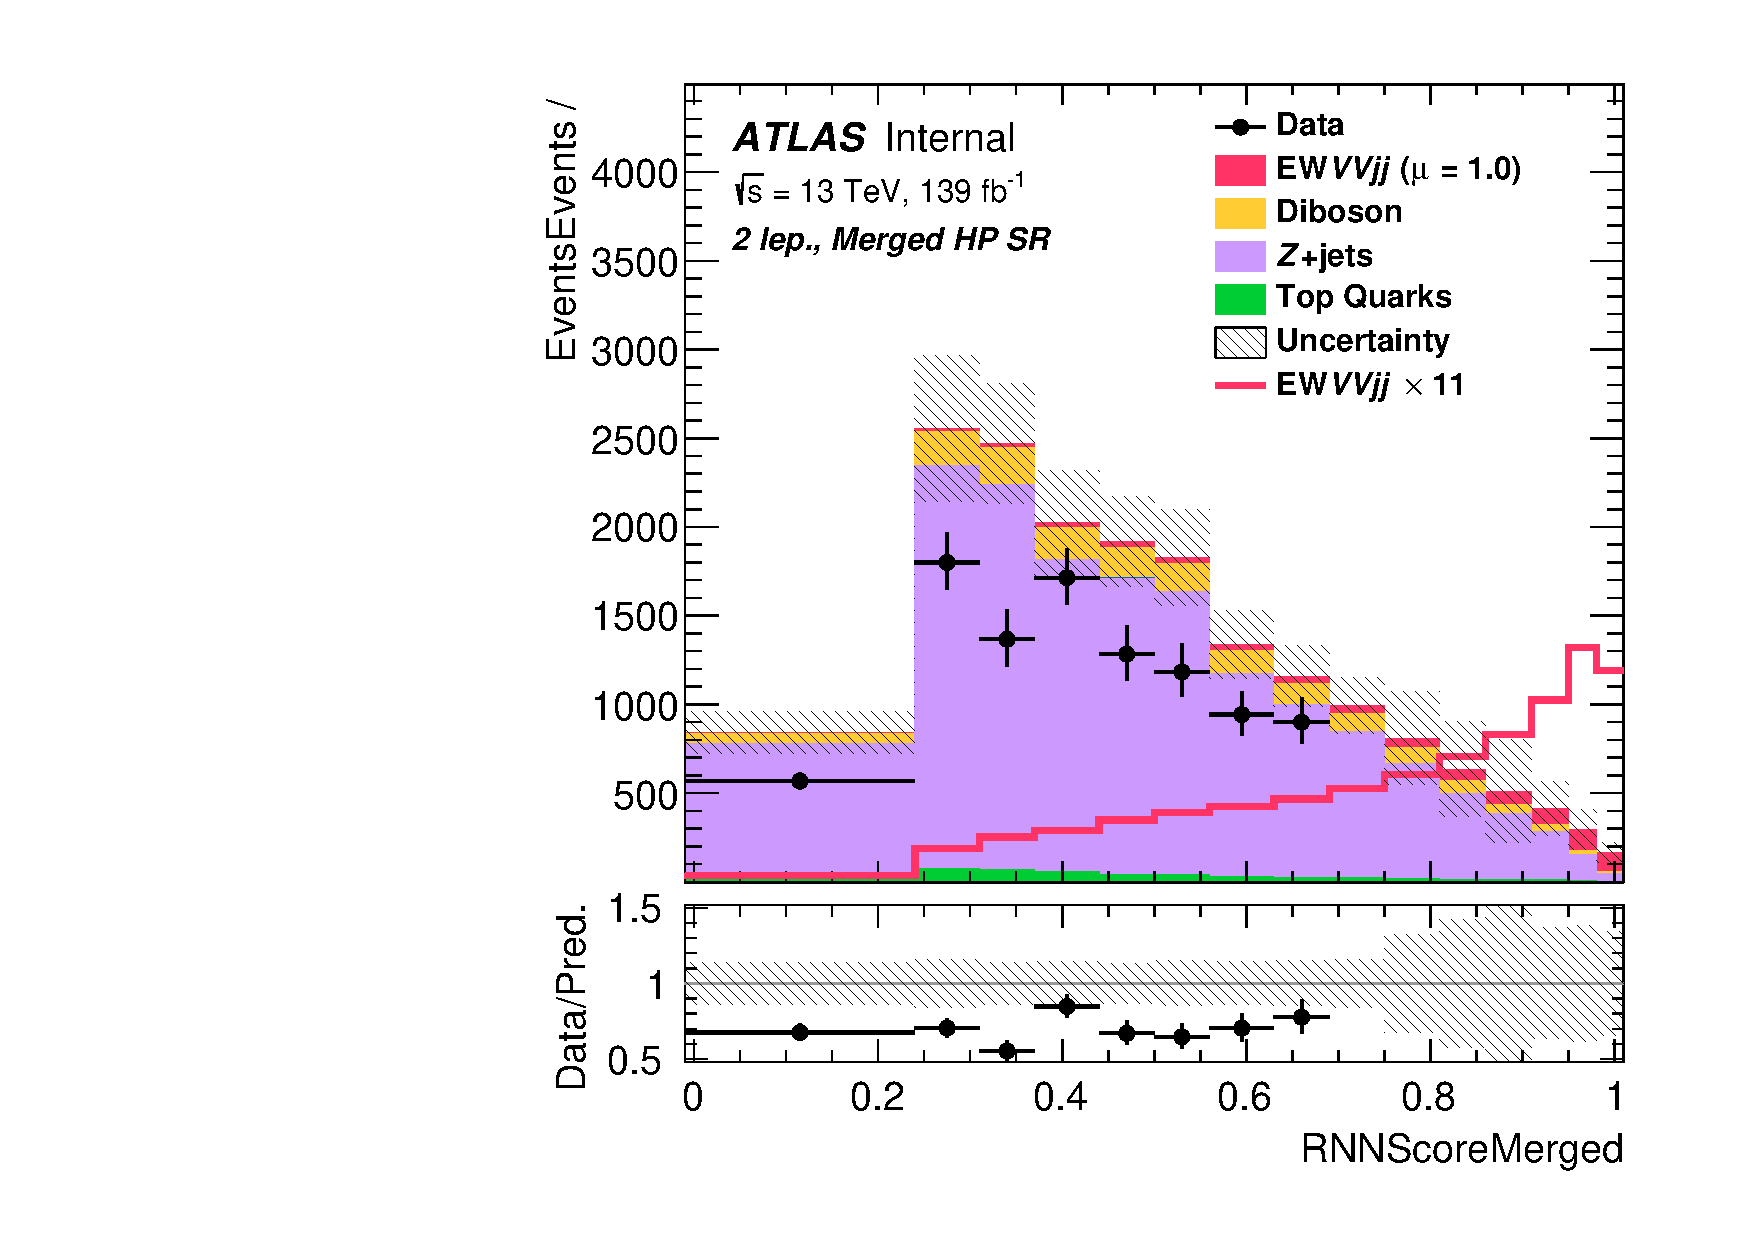
\includegraphics[width=0.35\textwidth]{figures/2lep/FitResults/Region_distRNNScoreMerged_DSRVBSHP_BMin0_J0_incJet1_L2_T0_incFat1_Y6051_incTag1_Fat1_Prefit.pdf}
    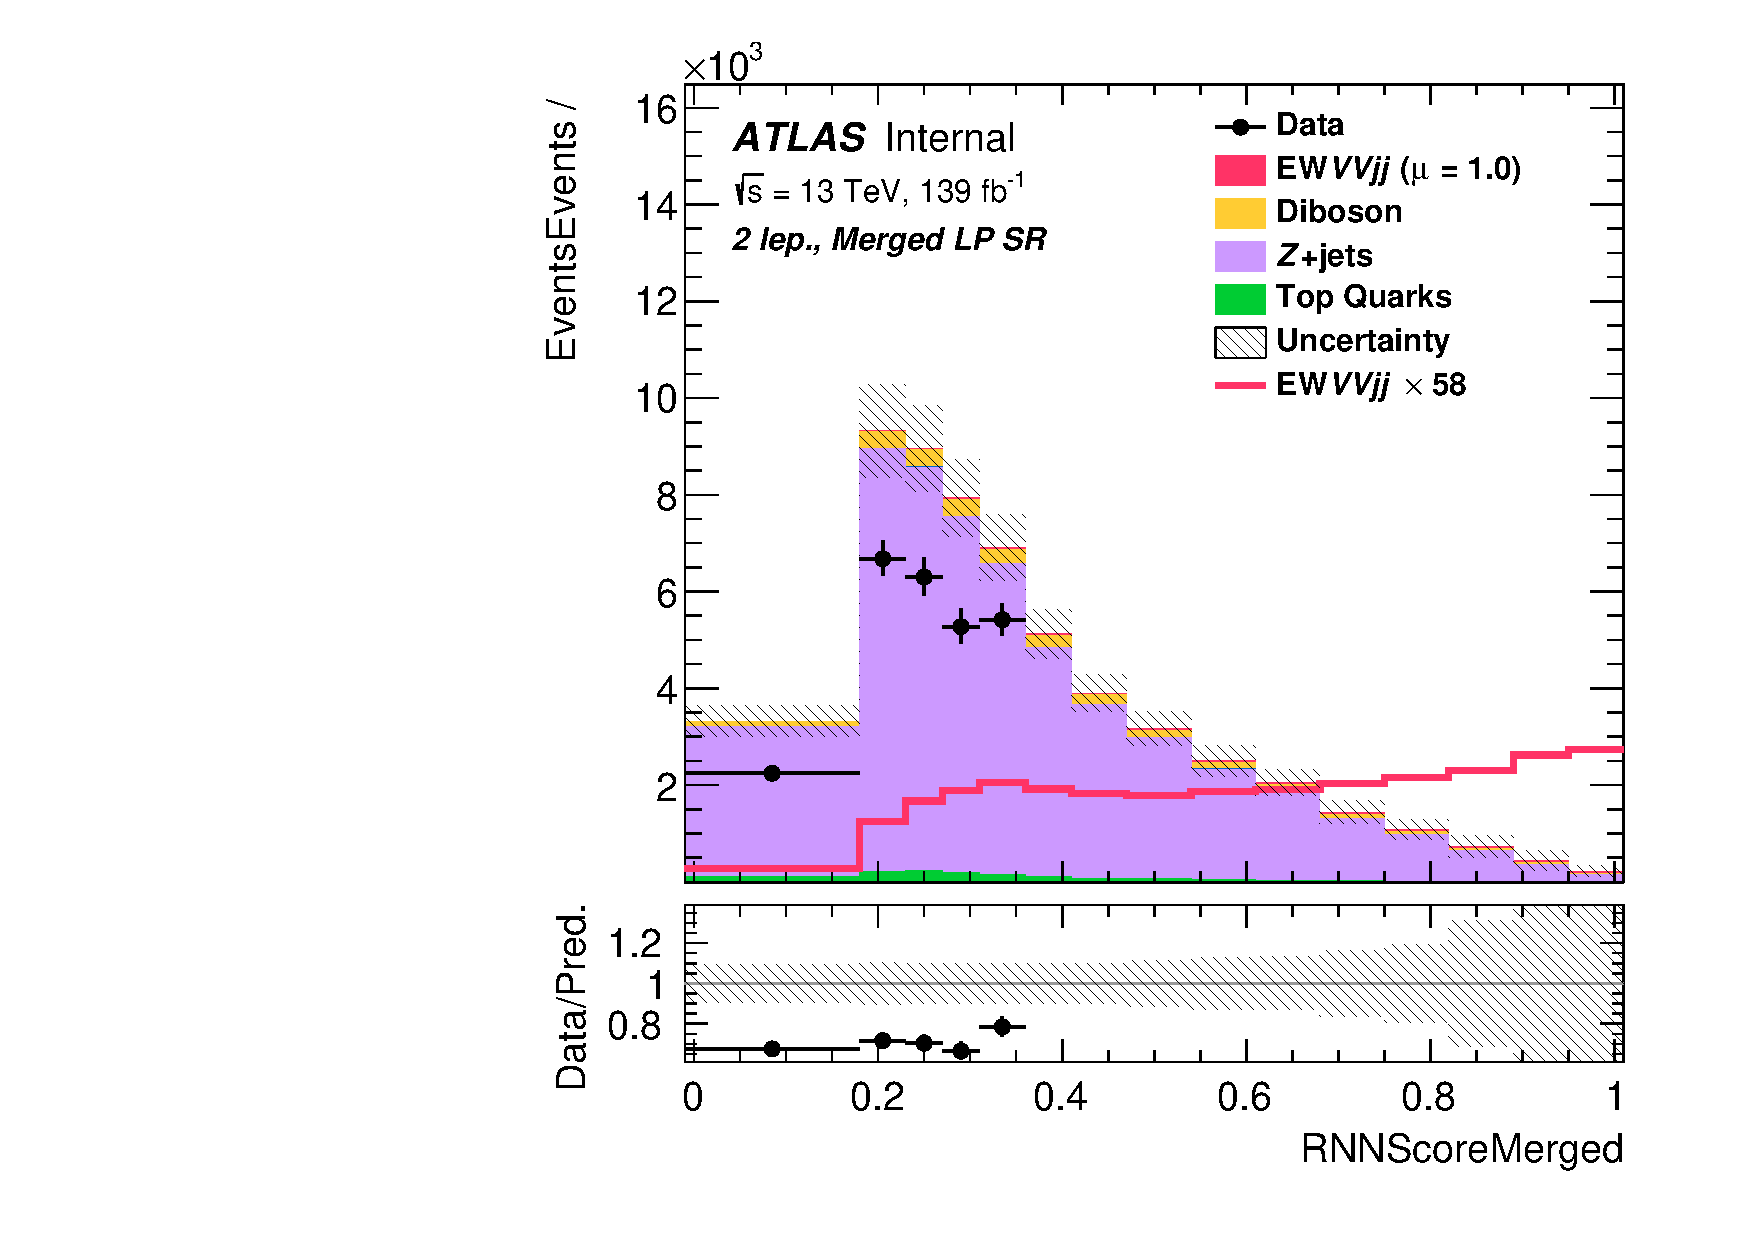
\includegraphics[width=0.35\textwidth]{figures/2lep/FitResults/Region_distRNNScoreMerged_DSRVBSLP_BMin0_J0_incJet1_L2_T0_incFat1_Y6051_incTag1_Fat1_Prefit.pdf}
    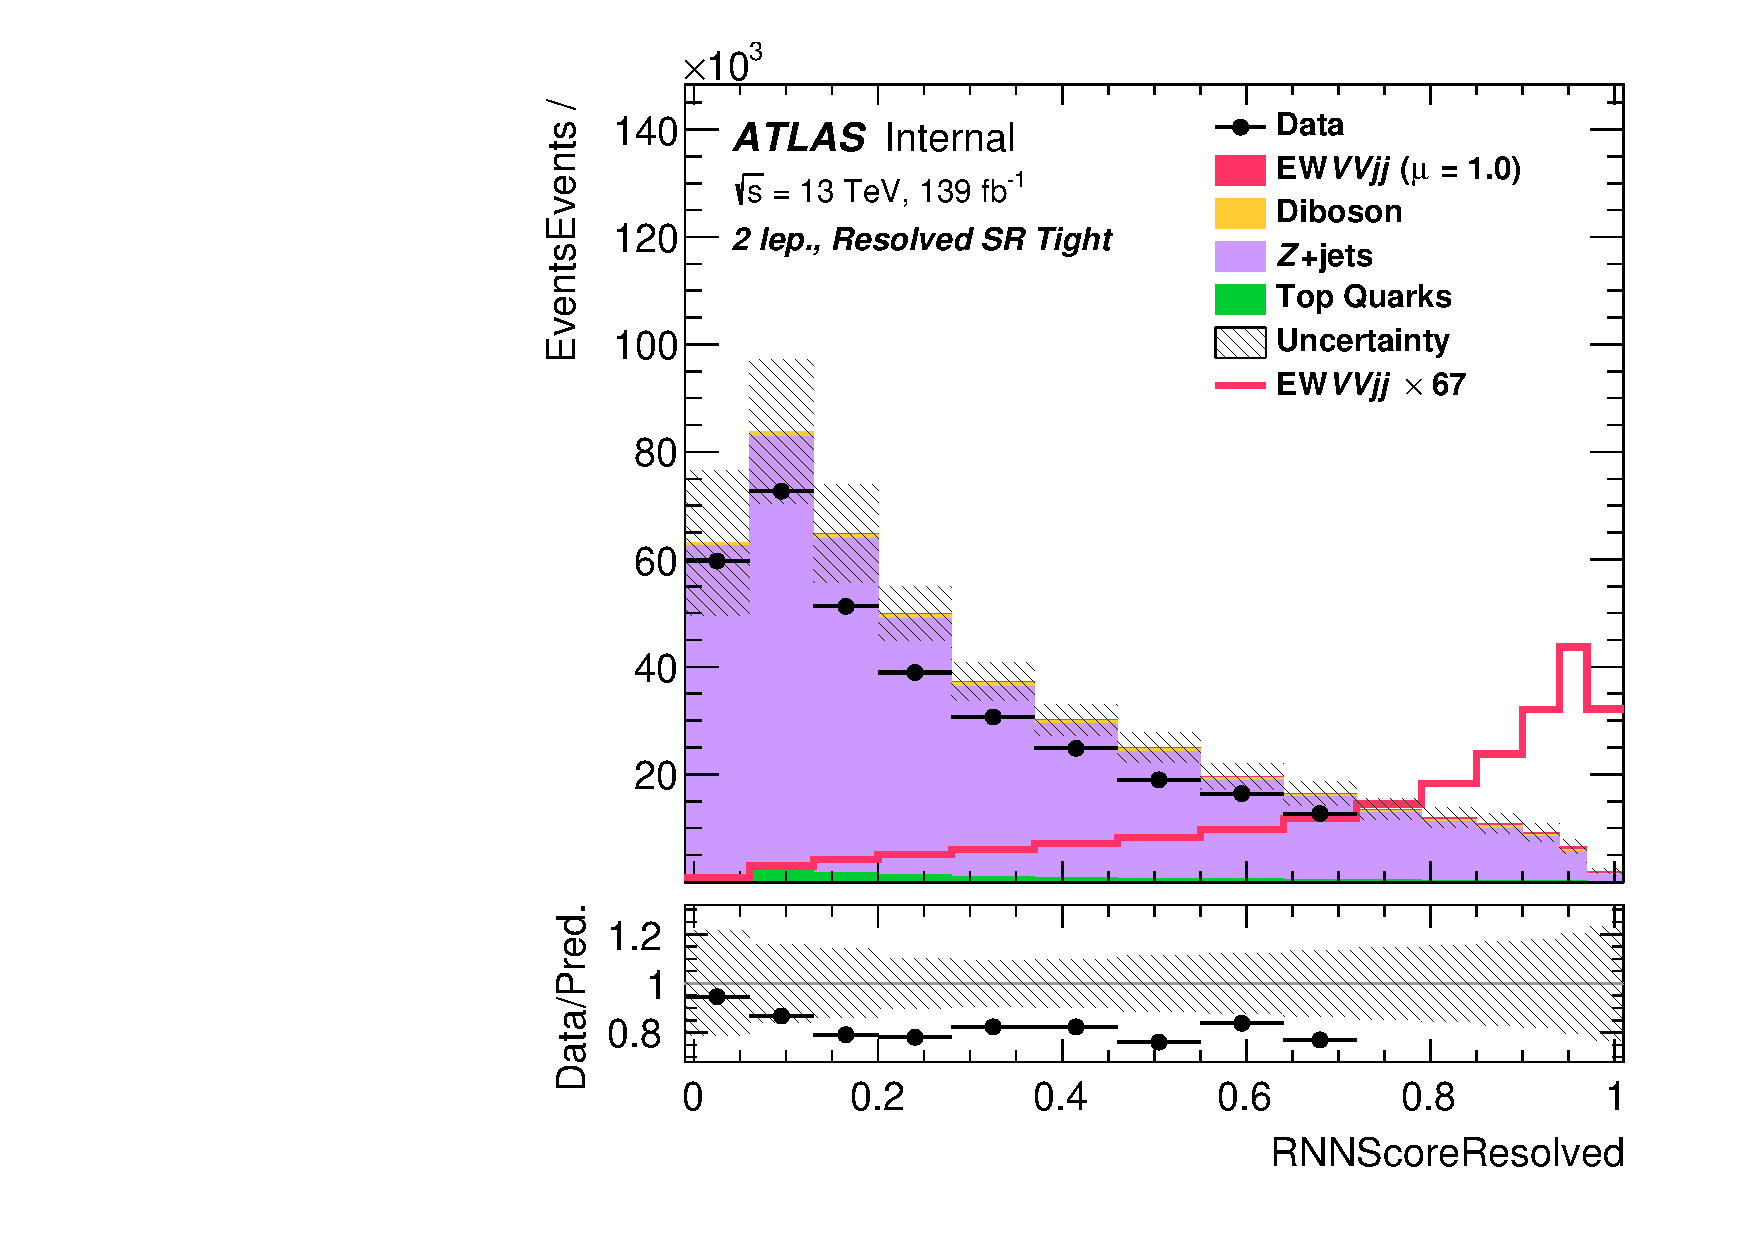
\includegraphics[width=0.35\textwidth]{figures/2lep/FitResults/Region_distRNNScoreResolved_DSRVBSFid_BMin0_T0_Y6051_incTag1_J2_L2_incJet1_Prefit.pdf}
    \\
    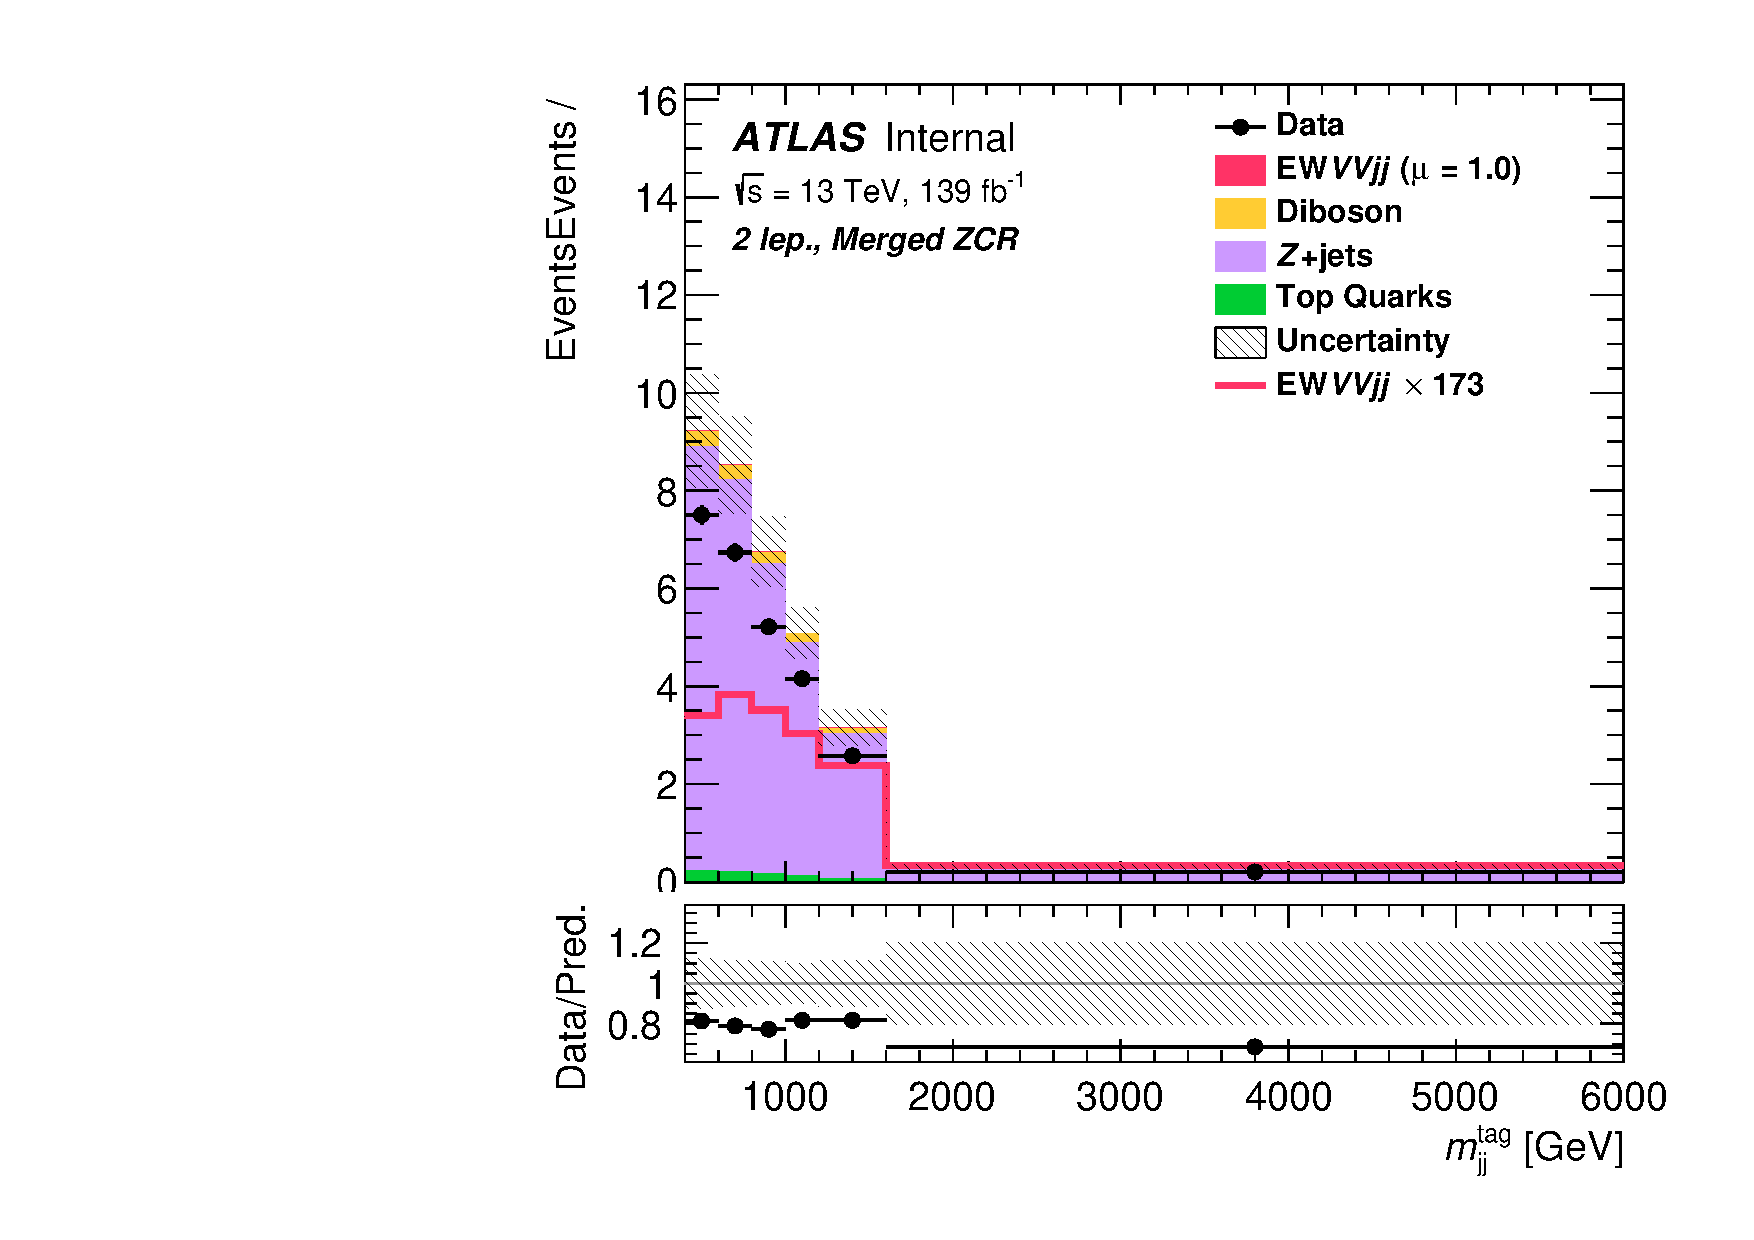
\includegraphics[width=0.35\textwidth]{figures/2lep/FitResults/Region_distMTagMerJets_DCRVjet_BMin0_J0_incJet1_L2_T0_incFat1_Y6051_incTag1_Fat1_Prefit.pdf}
    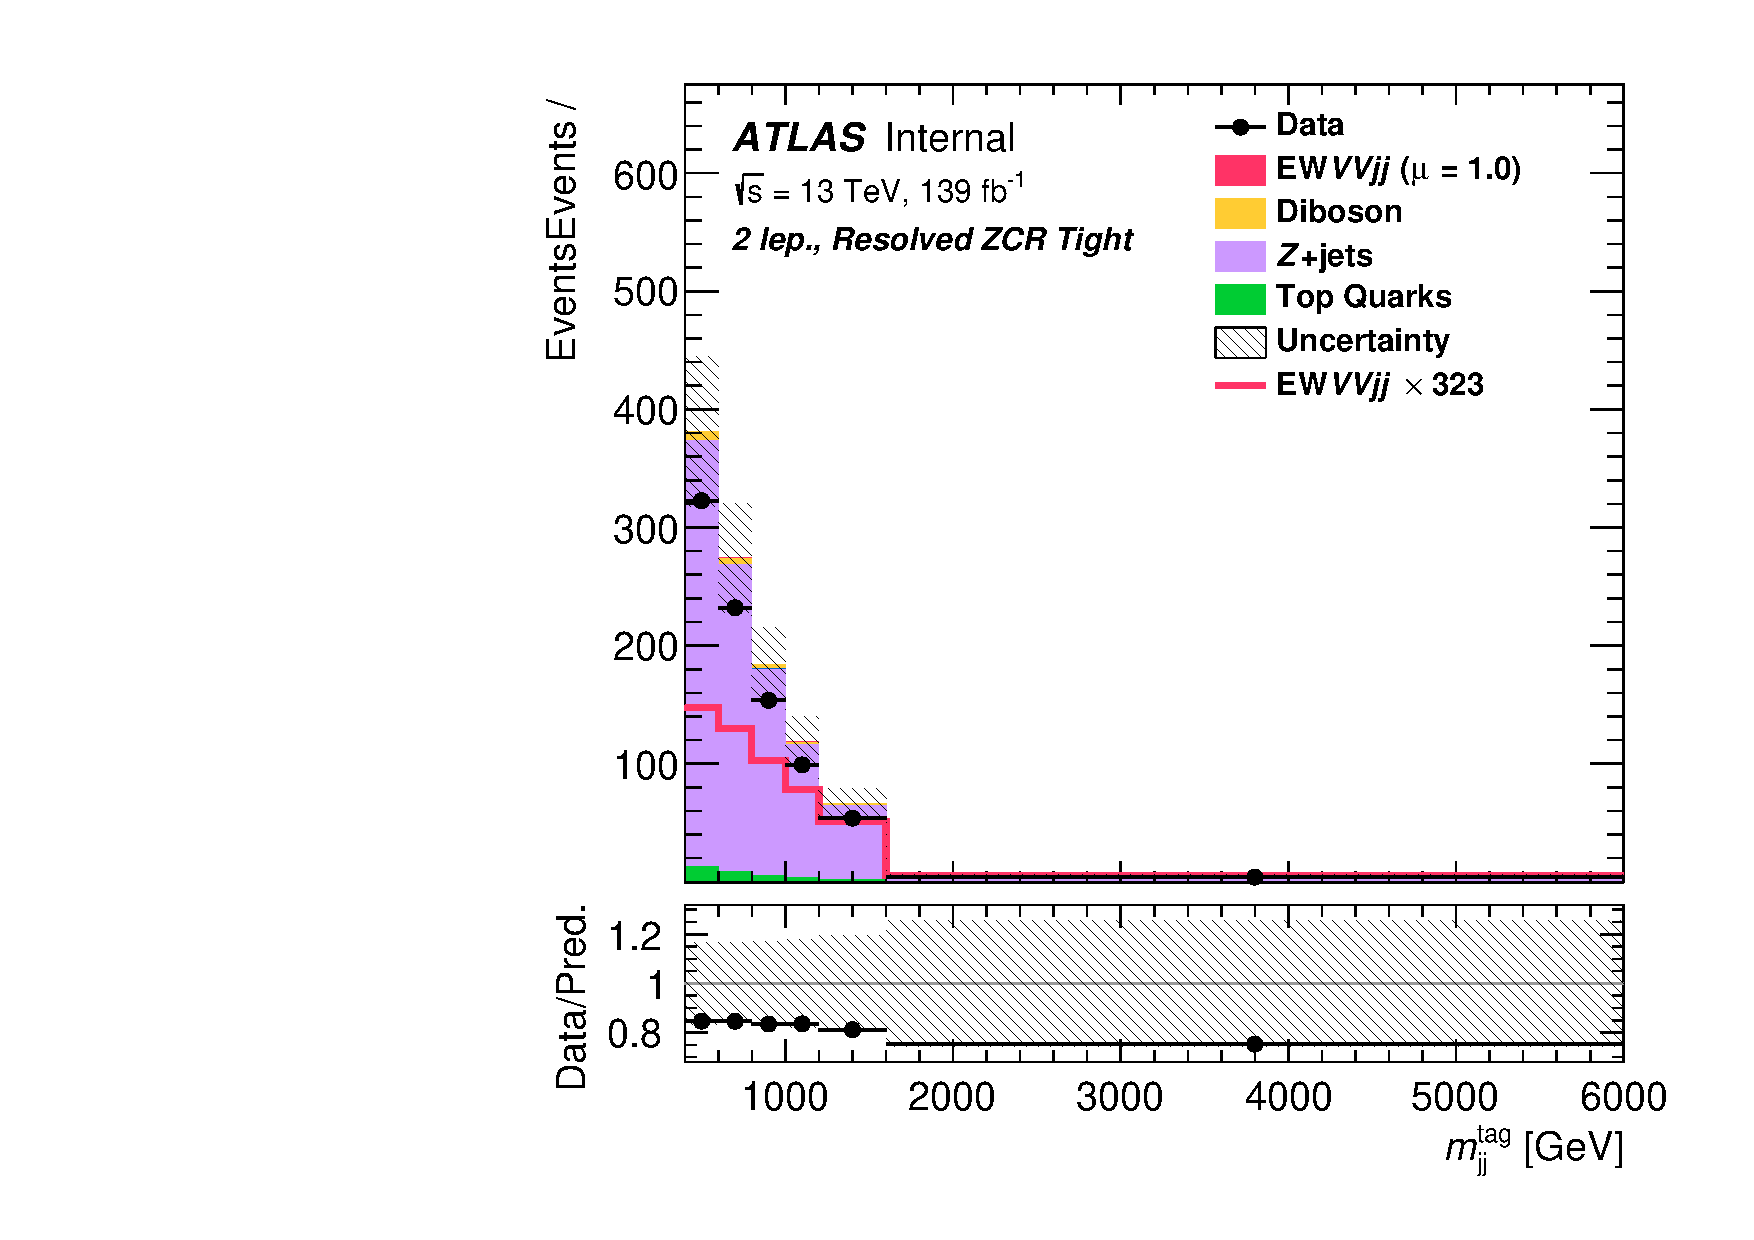
\includegraphics[width=0.35\textwidth]{figures/2lep/FitResults/Region_distMTagResJets_DCRVjetFid_BMin0_T0_Y6051_incTag1_J2_L2_incJet1_Prefit.pdf}
    \caption{Prefit plots for the 2 lepton channel. Data is blinded in the right bins that contain 75\% signal.}
       \label{fig:fit_2lep_prefit}
\end{figure}

\section{Postfit plots}
Figure~\ref{fig:fit_2lep_postfit} shows the post-fit plots of the analysis regions entering in the 2-lep fit only model. 
The fit is performed with only the left-bins, which are the bins that contain only 75\% signal.
In general, good agreement of the background prediction with the data within the uncertainty is observed after the fit even with only left-side bins. The discrepancy in the Z+jet background normalization  which is observed in the prefit plots seem to be fitted successfully.

\begin{figure}[ht]
    \centering
    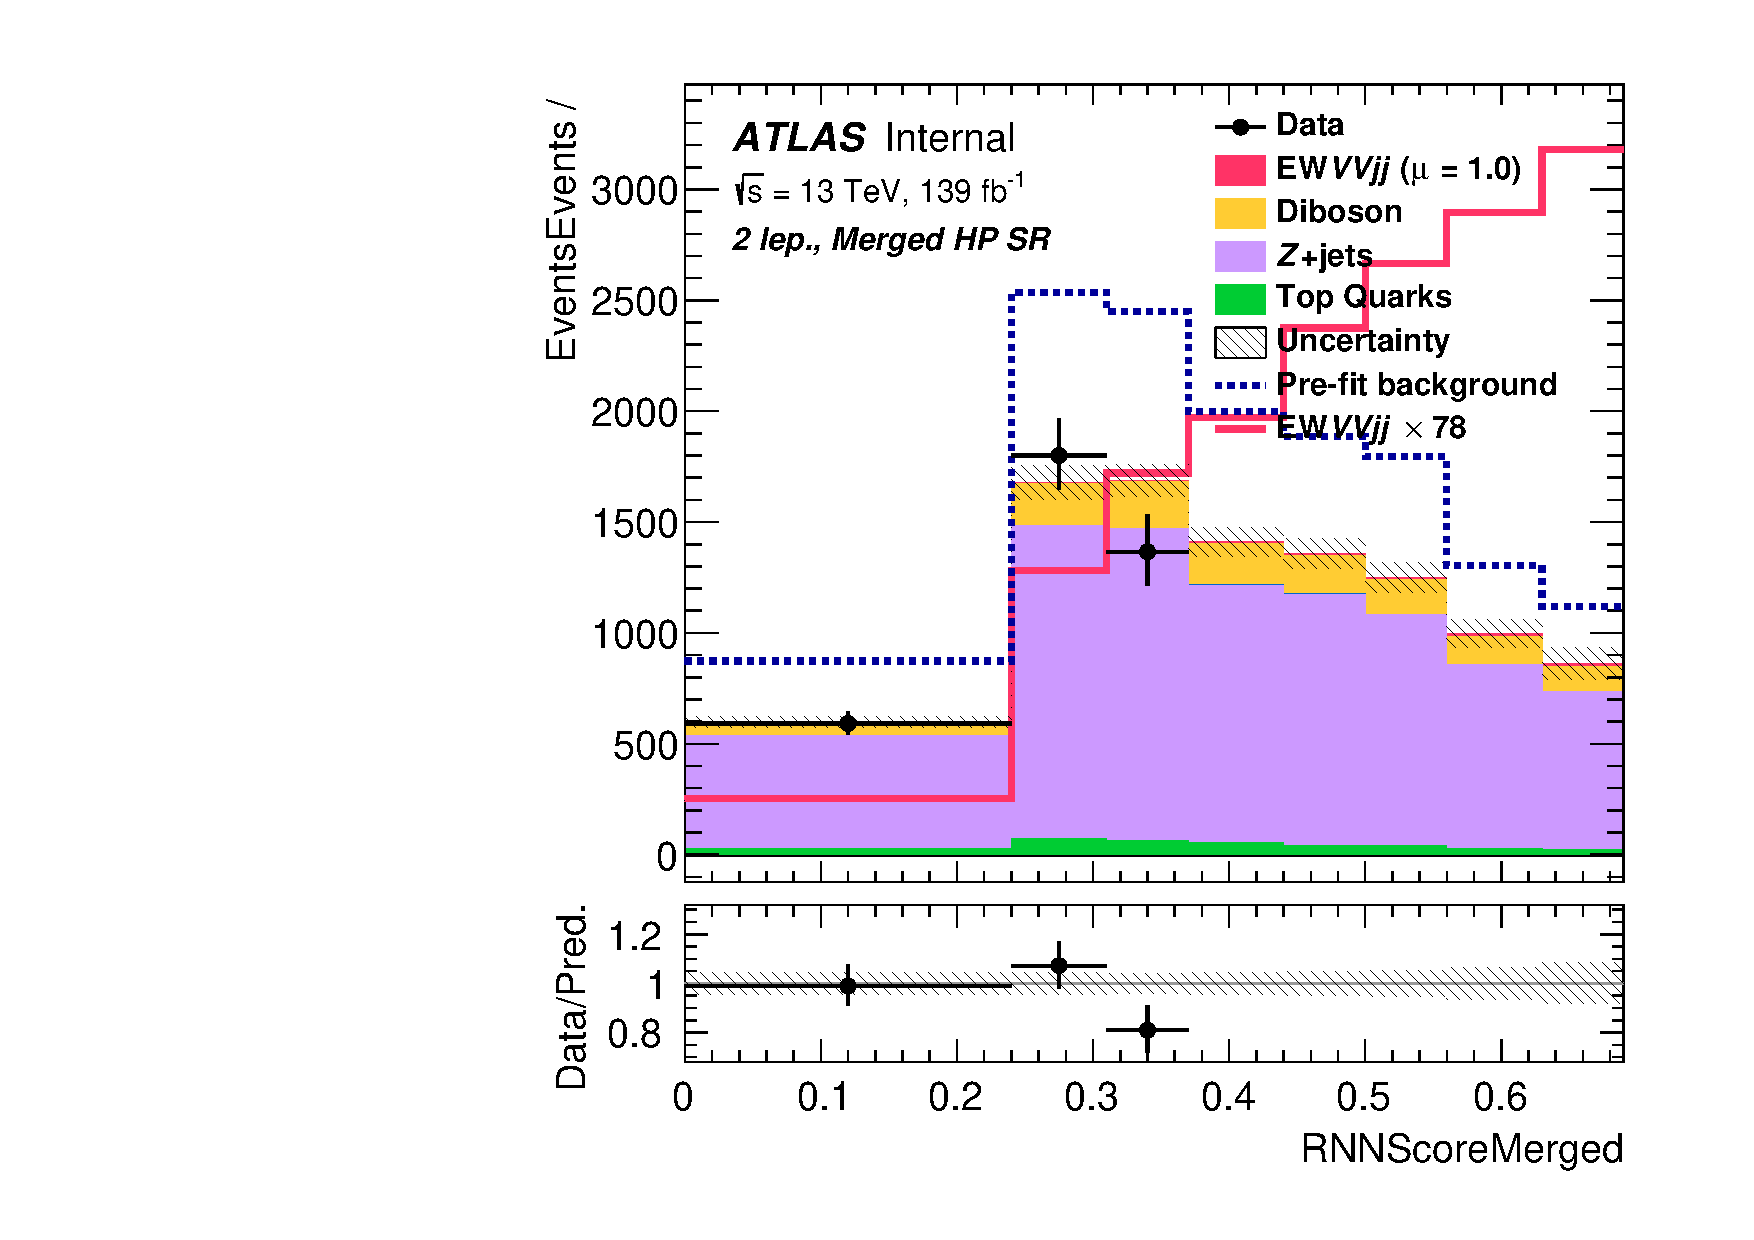
\includegraphics[width=0.35\textwidth]{figures/2lep/FitResults/Region_distRNNScoreMerged_DSRVBSHP_BMin0_J0_incJet1_L2_T0_incFat1_Y6051_incTag1_Fat1_GlobalFit_unconditionnal_mu1.pdf}
    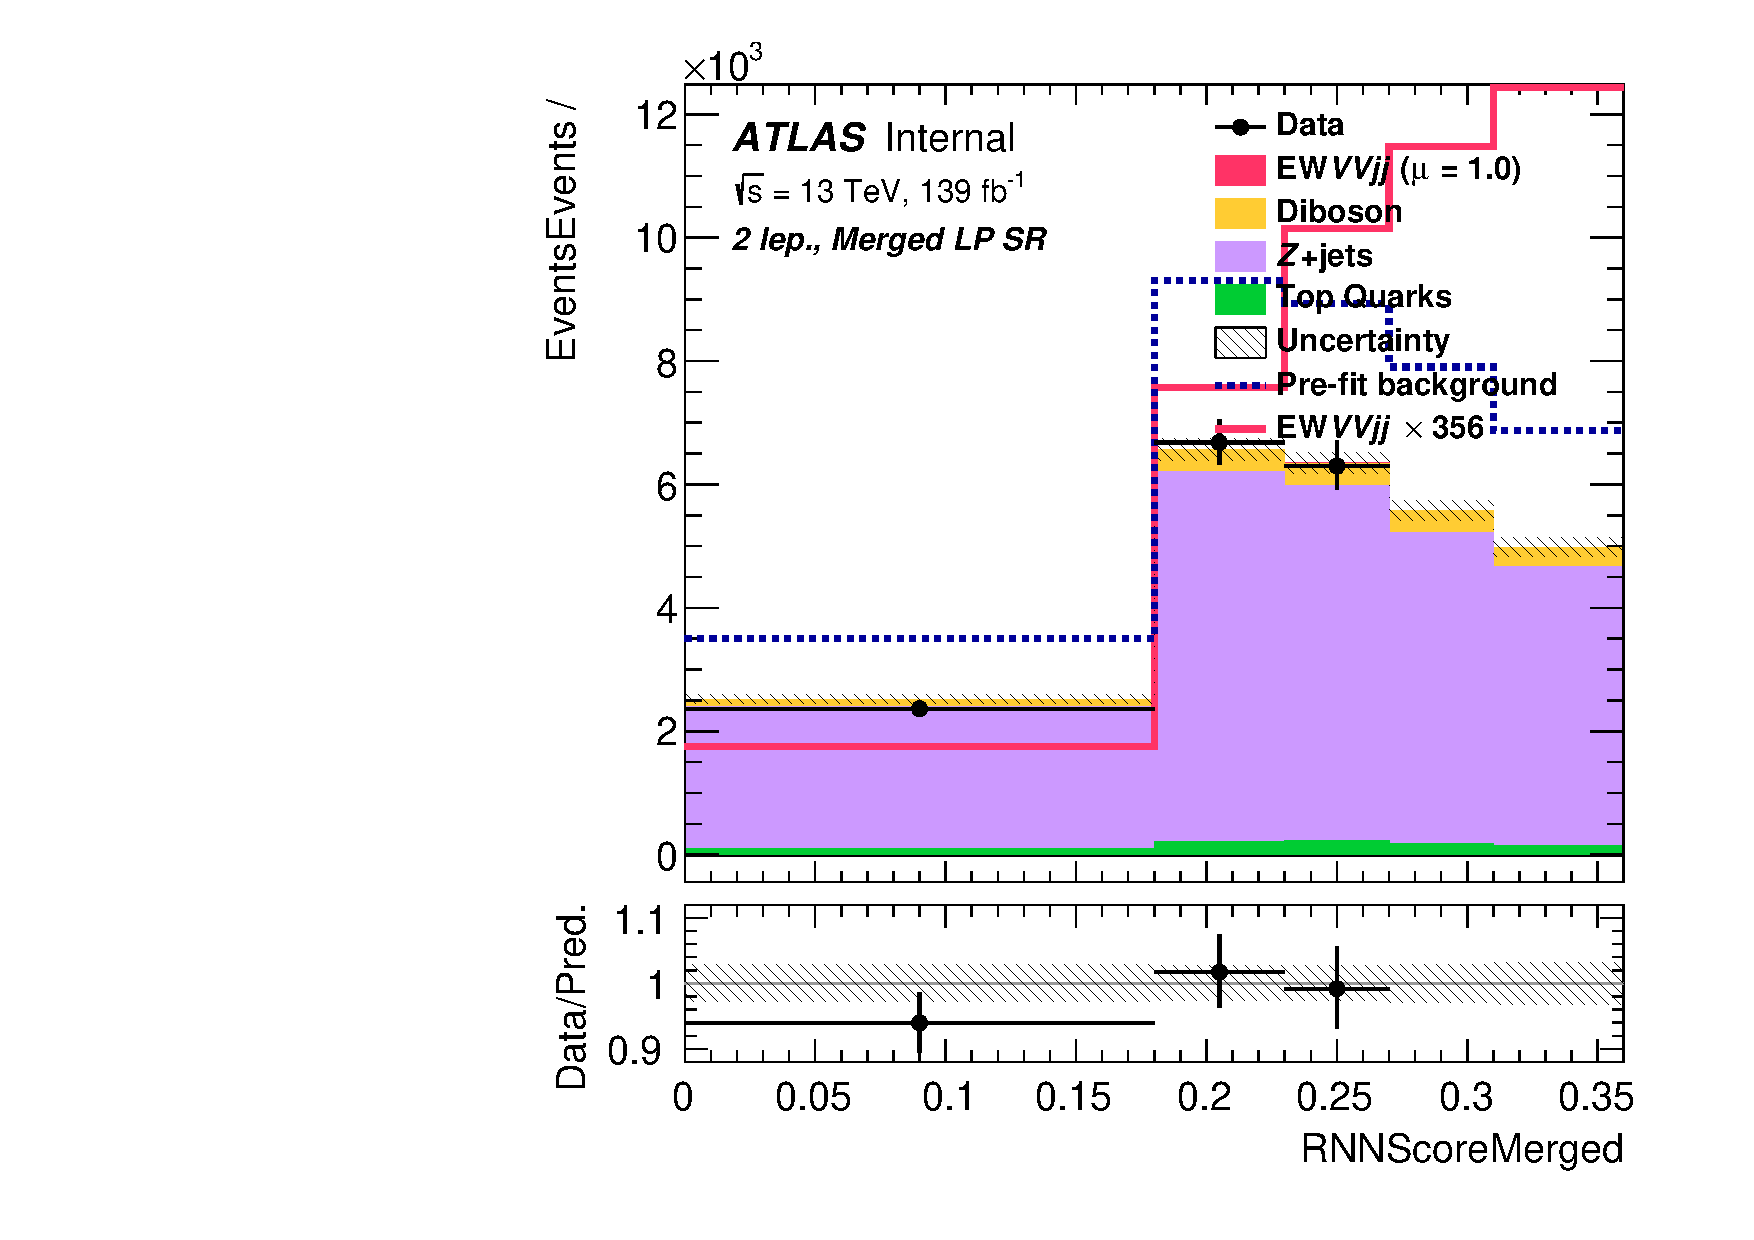
\includegraphics[width=0.35\textwidth]{figures/2lep/FitResults/Region_distRNNScoreMerged_DSRVBSLP_BMin0_J0_incJet1_L2_T0_incFat1_Y6051_incTag1_Fat1_GlobalFit_unconditionnal_mu1.pdf}
    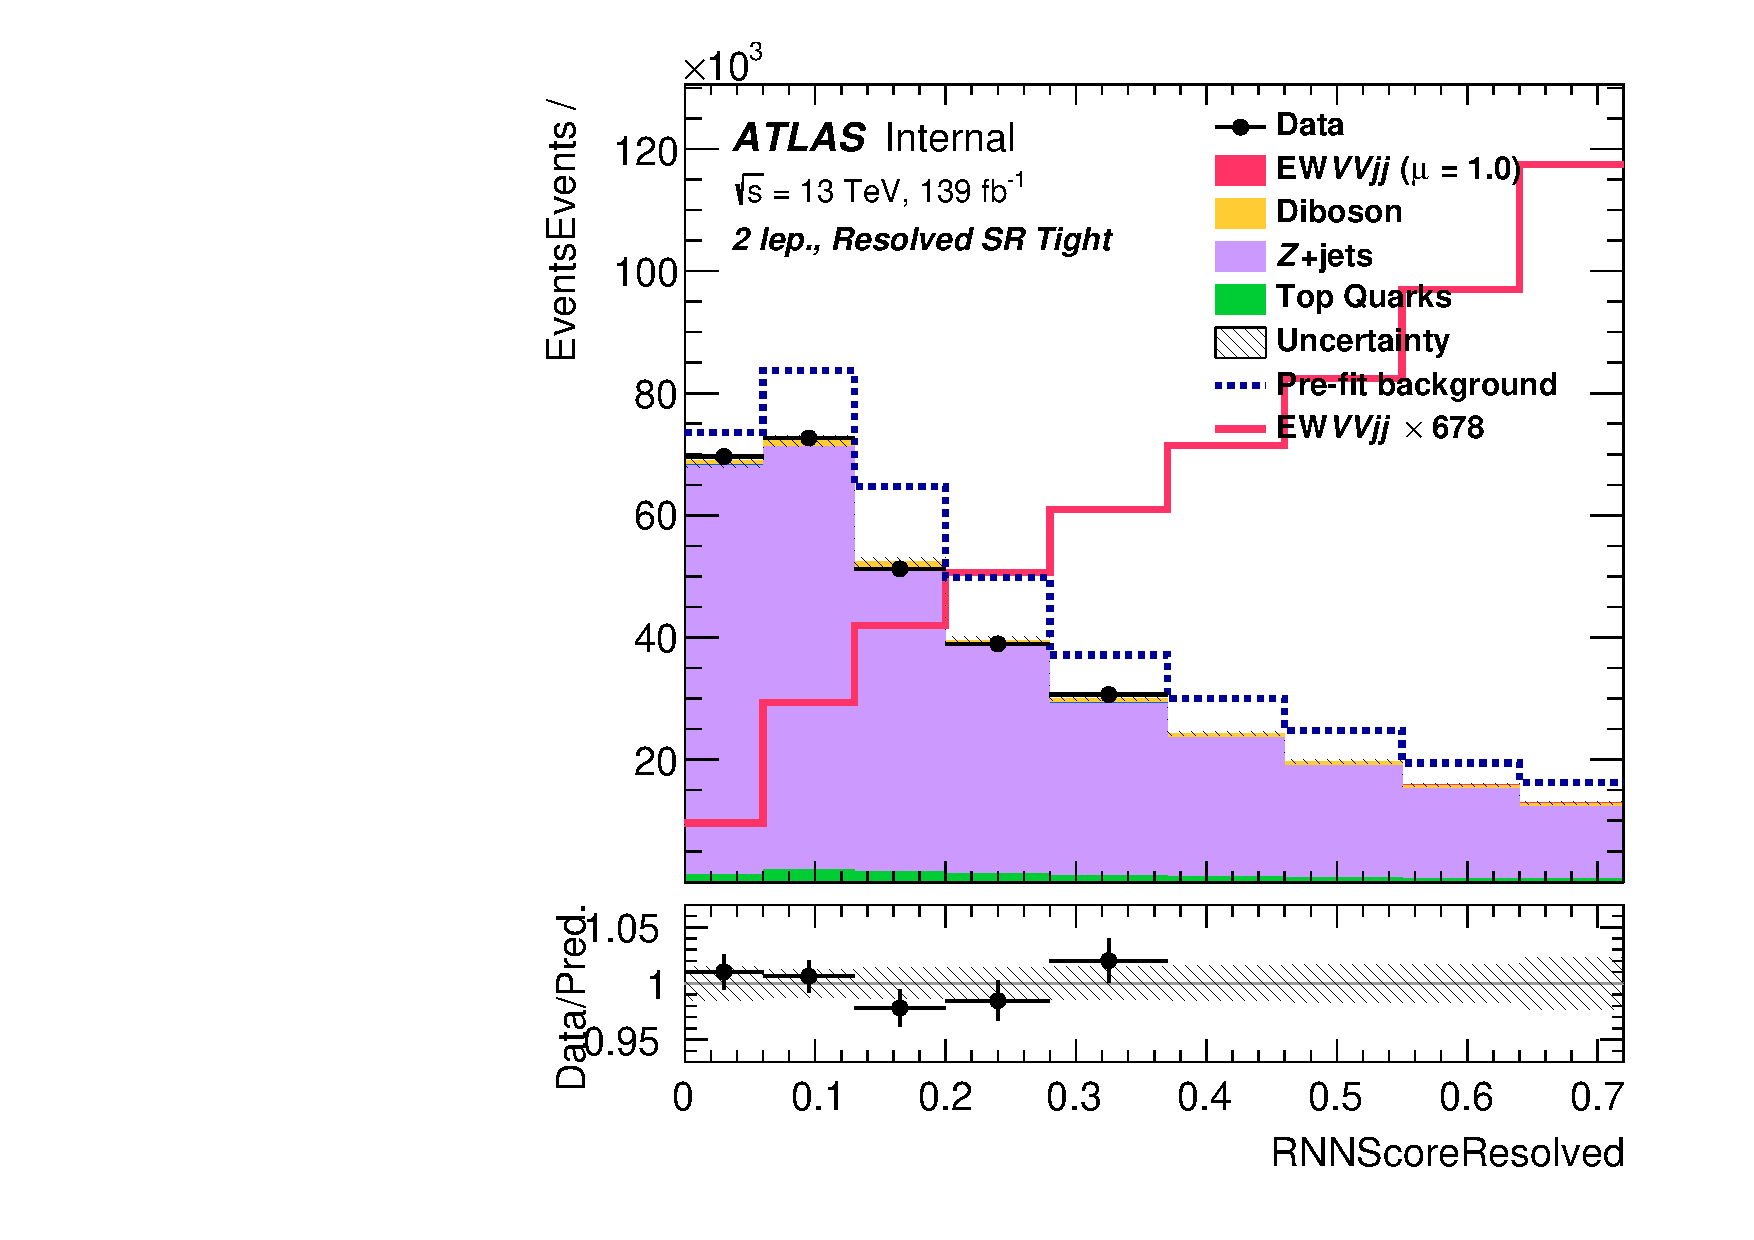
\includegraphics[width=0.35\textwidth]{figures/2lep/FitResults/Region_distRNNScoreResolved_DSRVBSFid_BMin0_T0_Y6051_incTag1_J2_L2_incJet1_GlobalFit_unconditionnal_mu1.pdf}
    \\
    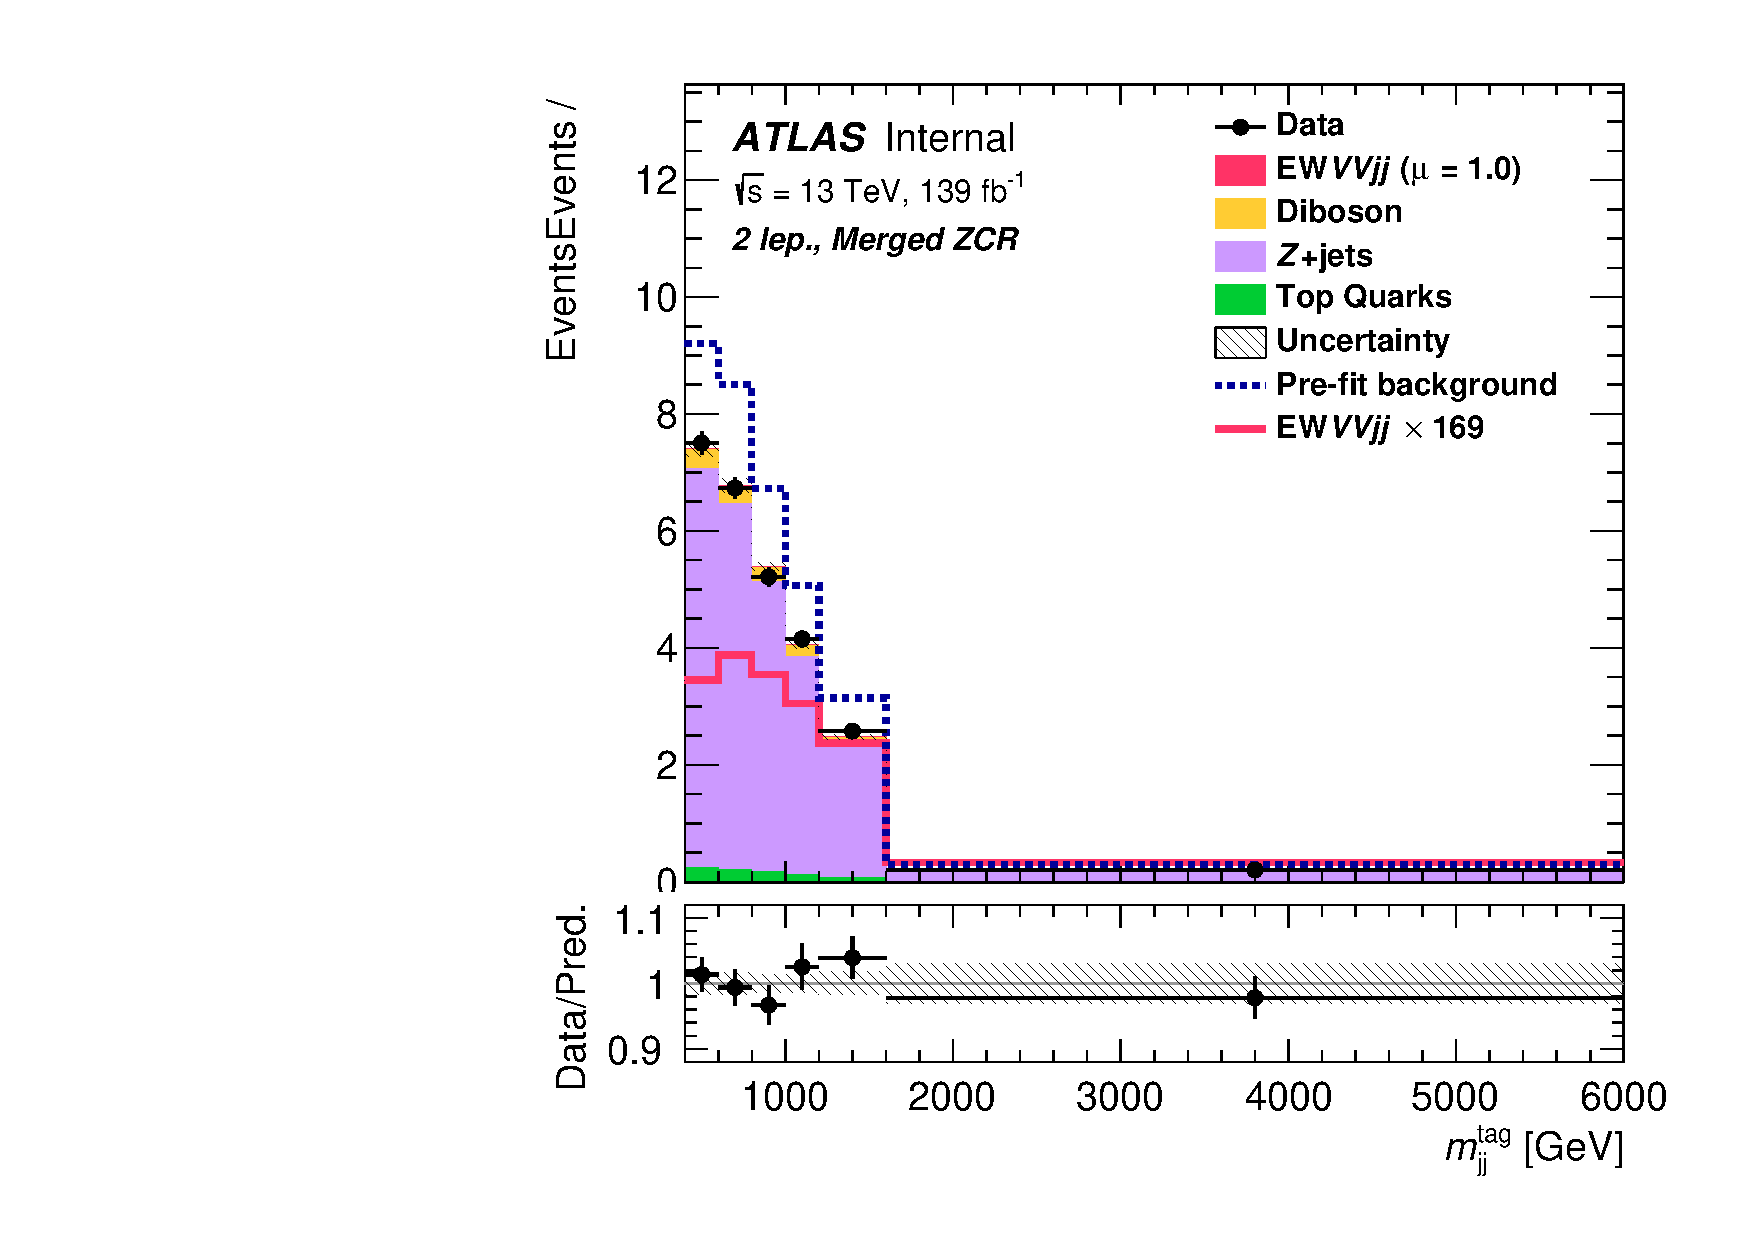
\includegraphics[width=0.35\textwidth]{figures/2lep/FitResults/Region_distMTagMerJets_DCRVjet_BMin0_J0_incJet1_L2_T0_incFat1_Y6051_incTag1_Fat1_GlobalFit_unconditionnal_mu1.pdf}
    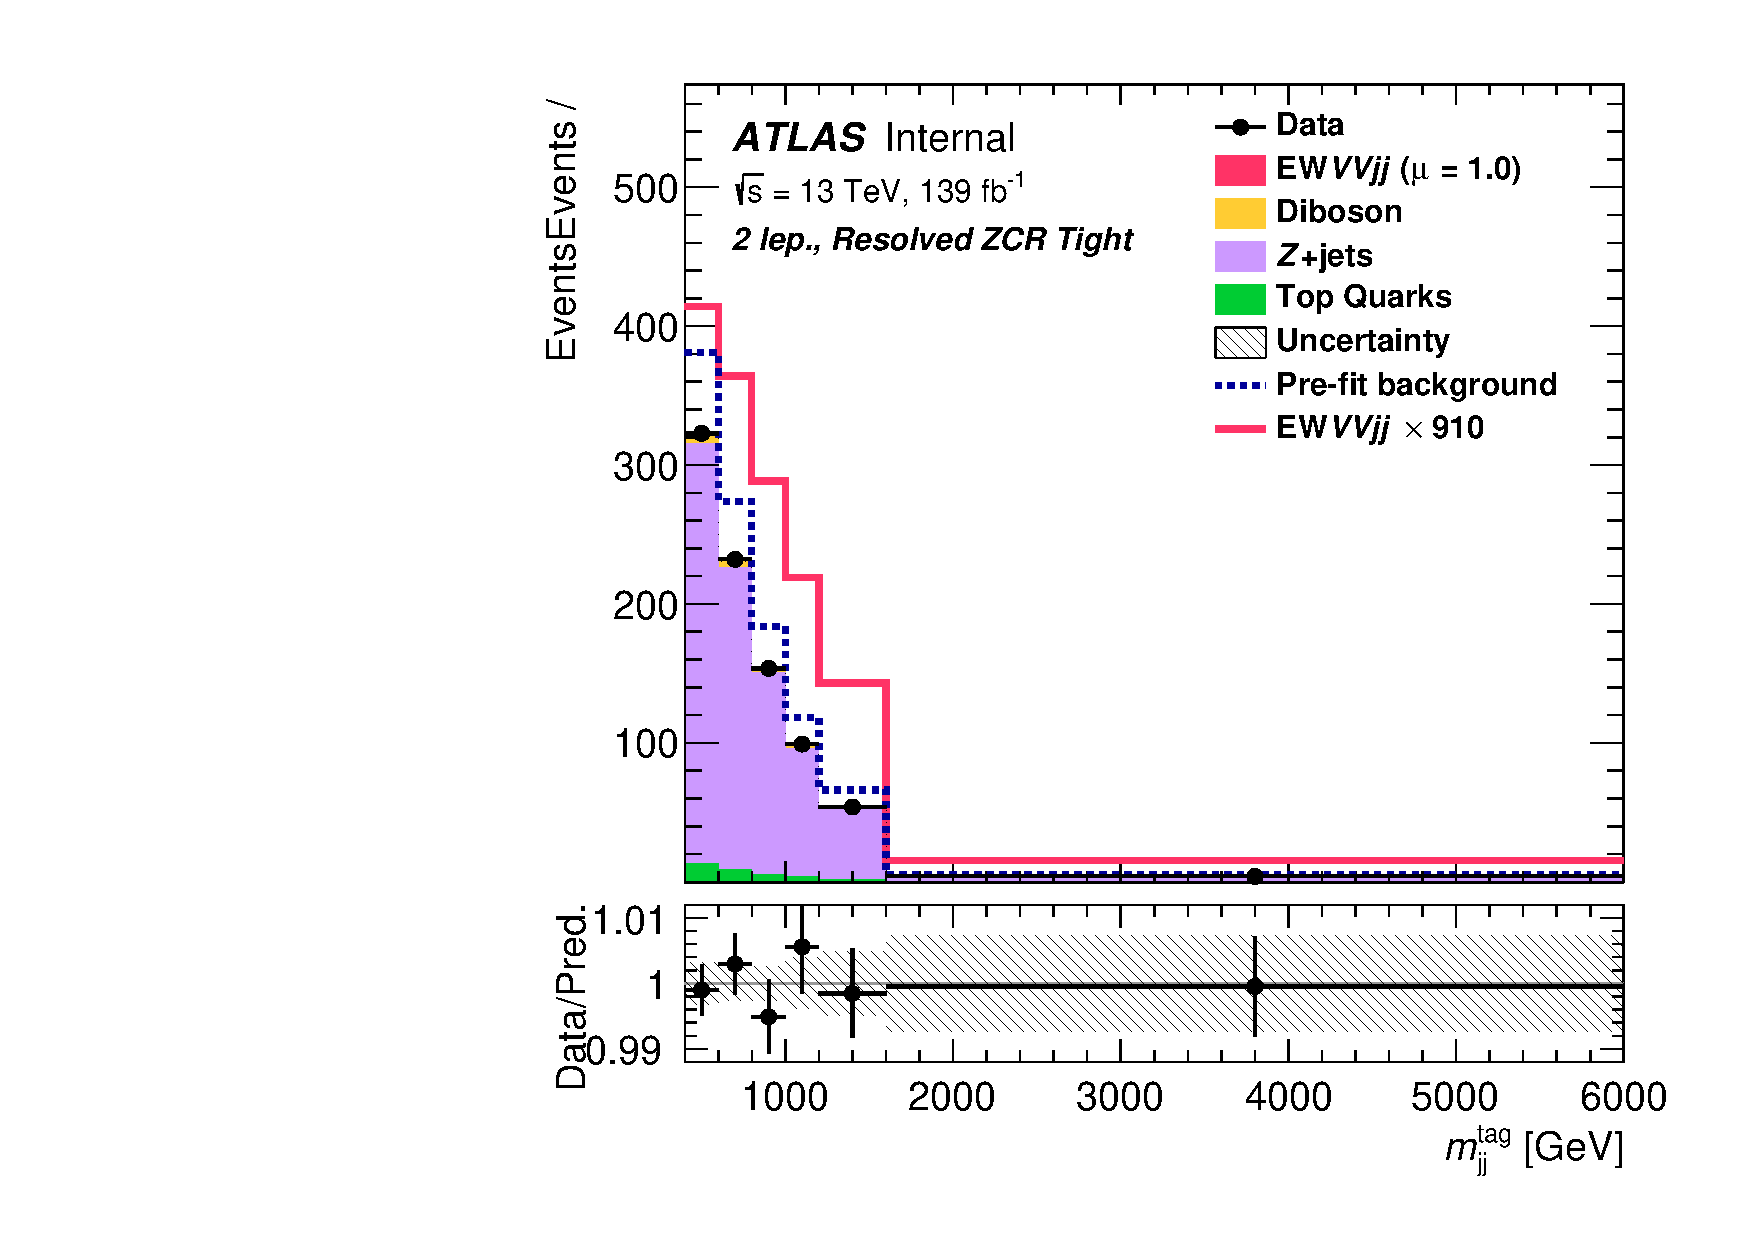
\includegraphics[width=0.35\textwidth]{figures/2lep/FitResults/Region_distMTagResJets_DCRVjetFid_BMin0_T0_Y6051_incTag1_J2_L2_incJet1_GlobalFit_unconditionnal_mu1.pdf}
    \caption{Postfit plots for the 2 lepton channel. Data is blinded in the right bins that contain 75\% signal.}
       \label{fig:fit_2lep_postfit}
\end{figure}

\section{Nuisance Parameter Pull}
The set of nuisance parameter pulls with Asimov dataset at full range is shown in picture~\ref{fig:fit_2lep_pullcomp}.
The pulls are compared to the fit of the left-side only bins, but also in Asimov dataset bins.
The strategy using only left-side bins, which include the 75\% of the signals from the right-most bins is adopted according to the unblinding strategy.
\begin{figure}[ht]
      \centering
        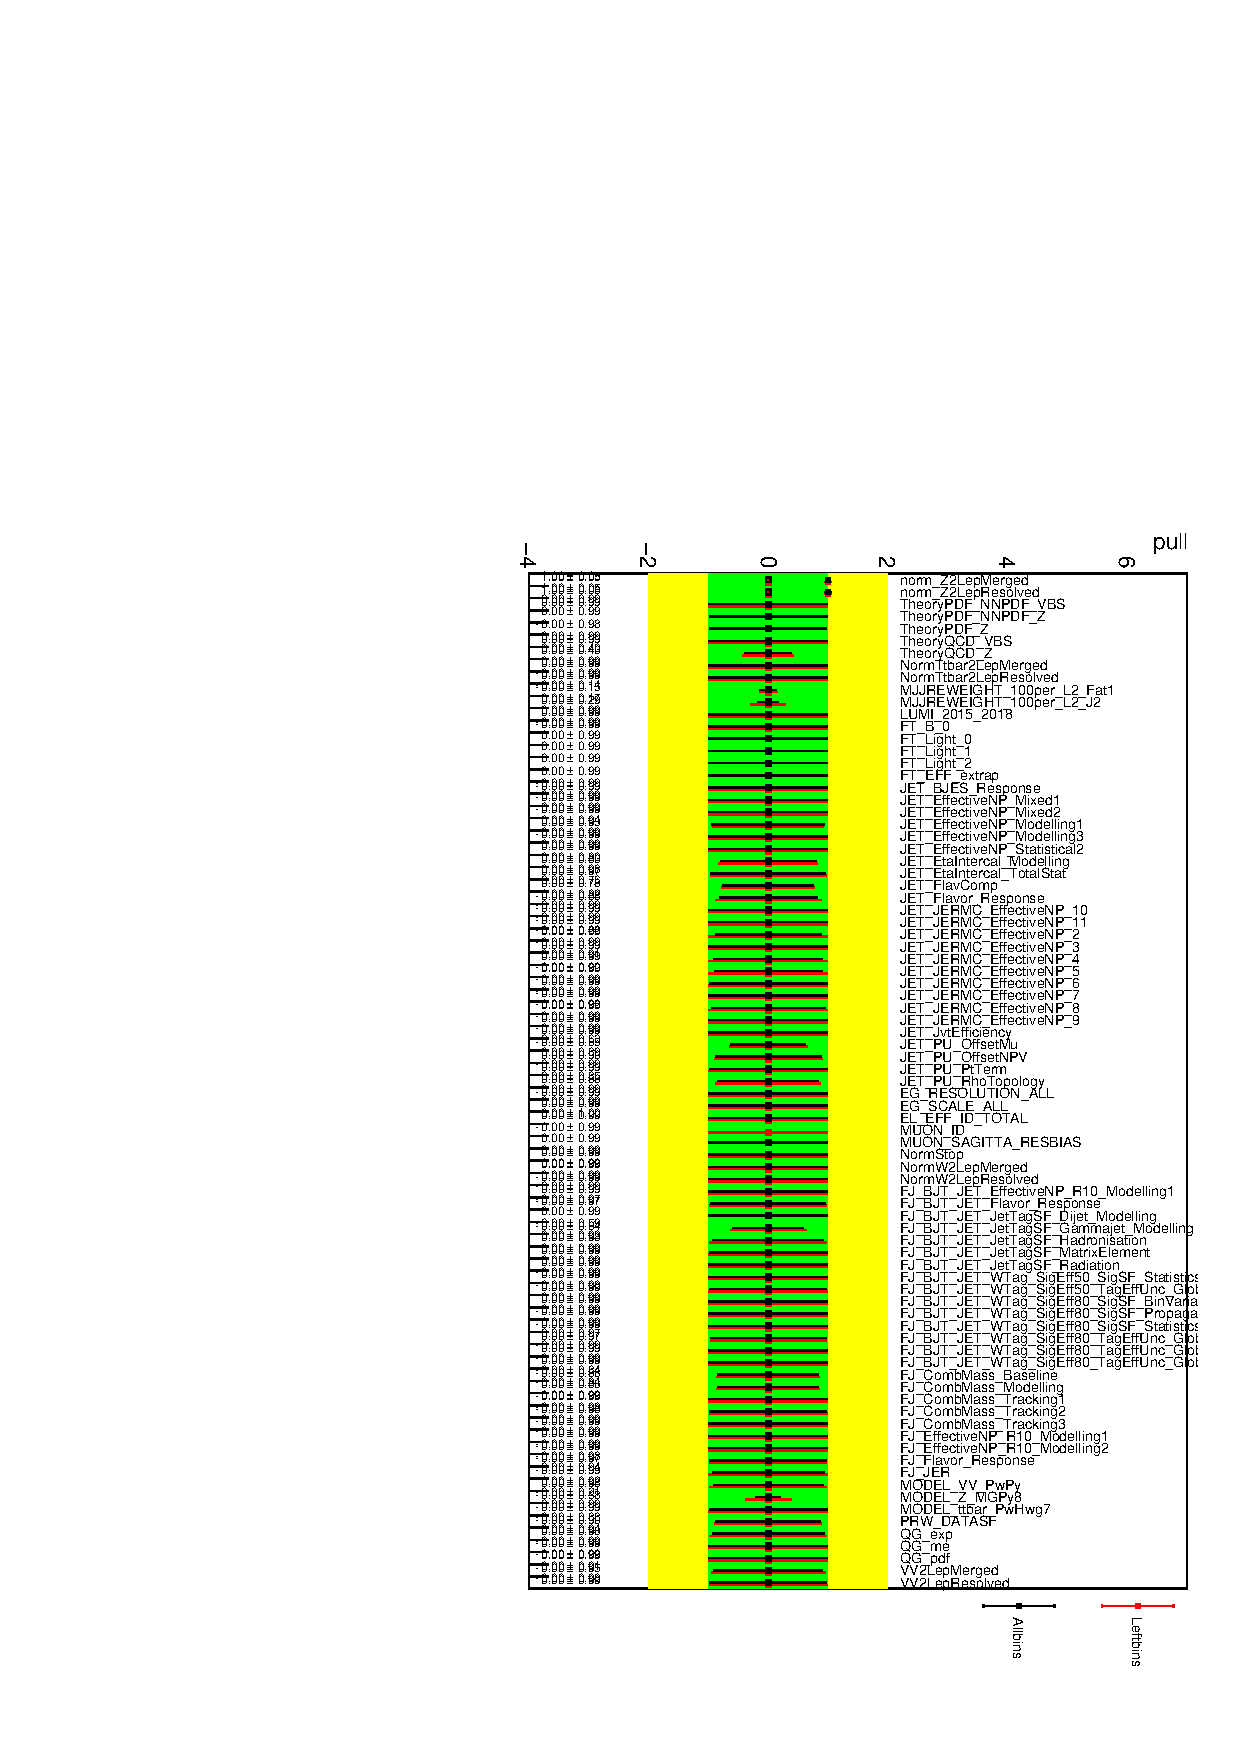
\includegraphics[width=0.8\textwidth]{figures/2lep/FitResults/fill_2lep_pullcomp.pdf}
        \caption{Fit cross-check, comparison of the unconditional fit to the data of only left-side bins and the unconditional fit ($\mu=1$) to Asimov data for the 2 lepton channel only.}
       \label{fig:fit_2lep_pullcomp}
\end{figure}
The nuisance parameters that constraints is similar between the full range and the left-side only bins. The unblinding strategy of using the The left-side only bins seems to work properly.\\

The set of nuisance parameter pulls from the fit to the data in the left-side bins is shown in Figure~\ref{fig:fit_2lep_pull}. The pulls are compared to the fit to the Asimov dataset, only for left-side bins similarly to the data fit. 
\begin{figure}[ht]
      \centering
        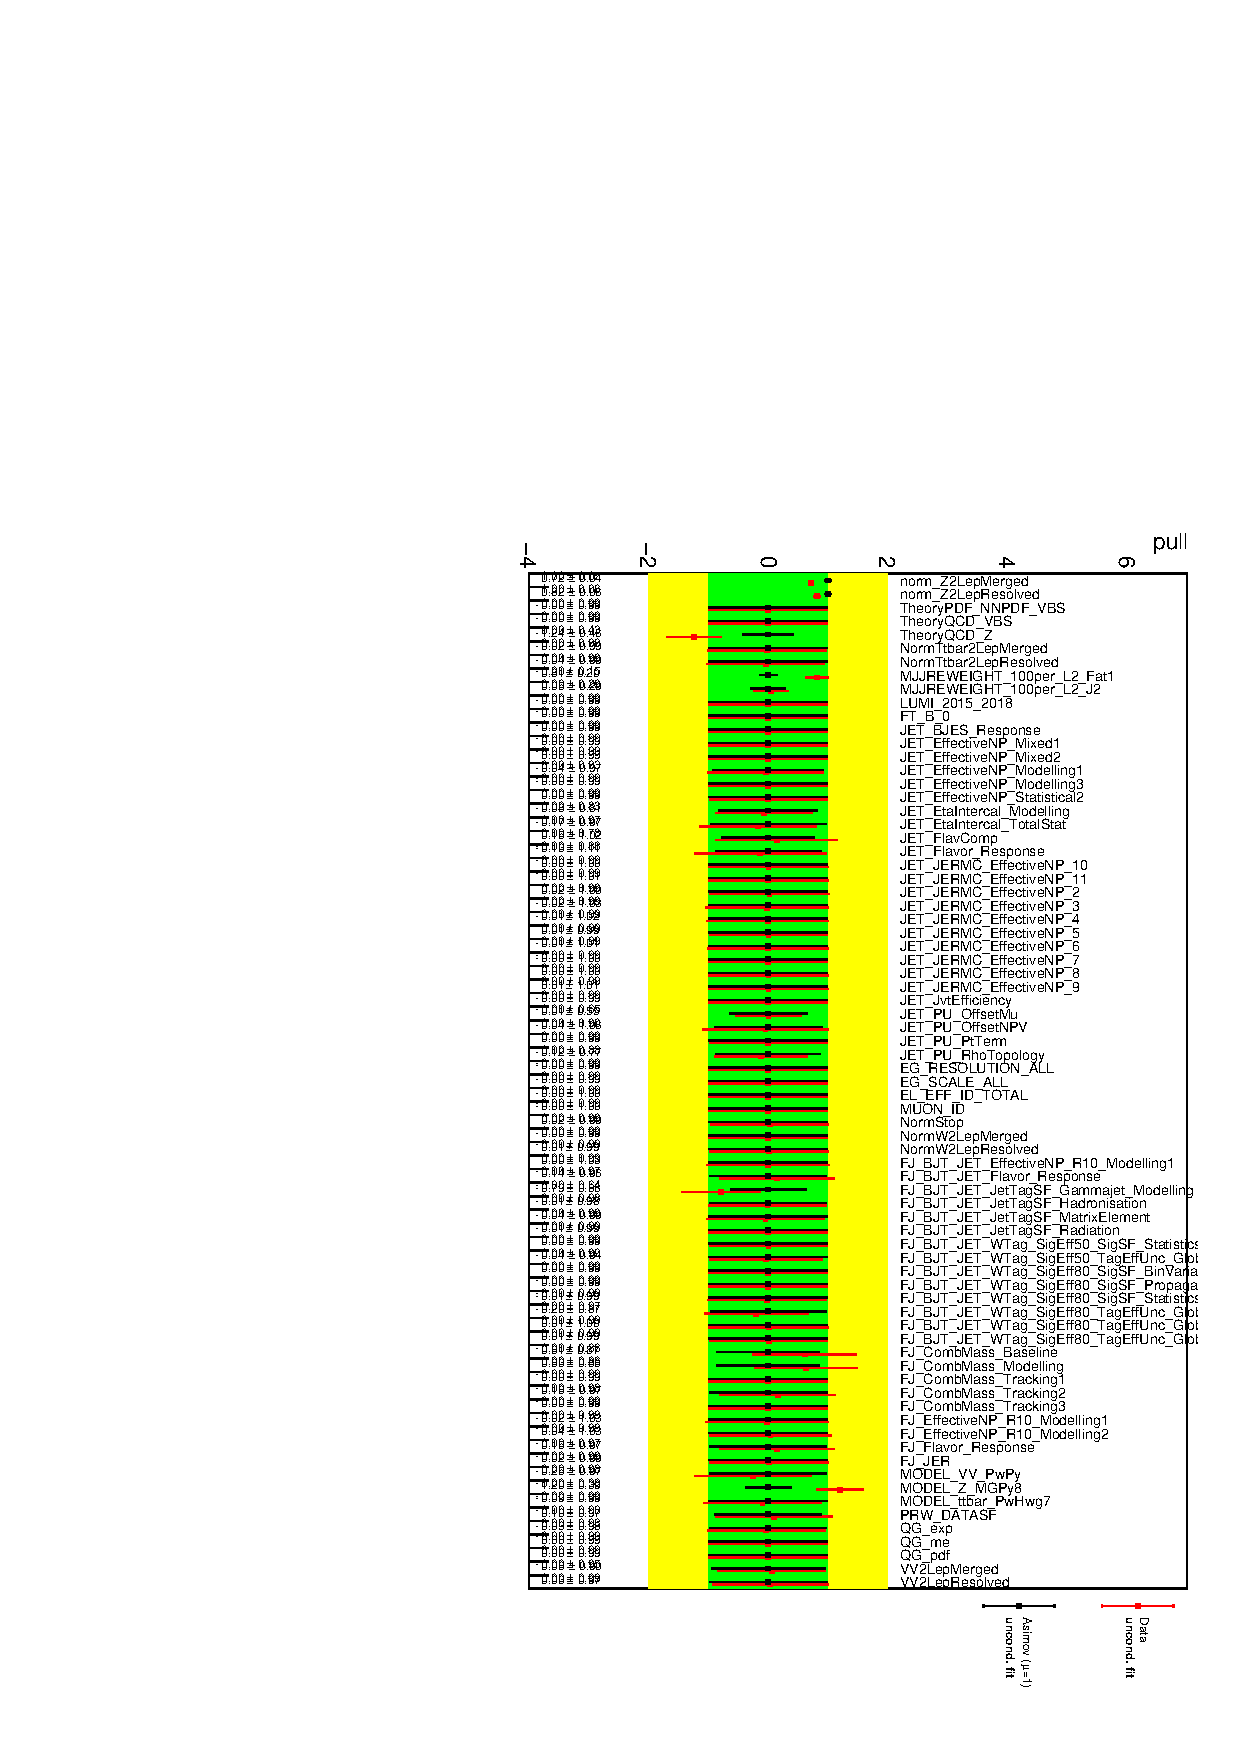
\includegraphics[width=0.8\textwidth]{figures/2lep/FitResults/fit_2lep_pull.pdf}
        \caption{Fit cross-check, comparison of the unconditional fit to the data of only left-side bins and the unconditional fit ($\mu=1$) to asimov data for the 2 lepton channel only.}
       \label{fig:fit_2lep_pull}
\end{figure}

The parameters are well behaved and most pulls are within the 1.5$\sigma$.
The parameters related to the normalizations of the backgrounds with priors are fitted within the range of the set prior, which is a good thing since otherwise the setting of the prior can be problematic.
The constrains shown in data left-side bins fit is similar to what is seen in Asimov dataset fit, which means the Asimov dataset seems to model the data well.
Most nuisance parameters are mildly constraints, exceptions are:
\begin{itemize}
       \item \texttt{SysTheoryQCD\_Z} 
        This is the QCD scale uncertainty for the Z+jets background sample. This comes from the large shape variation in the resolved SR. The input variations are shown in Figure and Figure in the merged and resolved SRs. \\
       \item \texttt{MJJREWEIGHT\_100per\_L2\_Fat1} 
       \item \texttt{MJJREWEIGHT\_100per\_L2\_J2} \\
       These are the $m^{tag}_{jj}$ reweighting uncertainties for merged and resolved regions. We expect the large constraints for these uncertainties since these are taken as 100\% uncertainties.Therefore CRs have large variations and constraints this systematics uncertainties. \\
       \item \texttt{SysMODEL\_Z\_MGPy8} \\
       This is the shape difference between Sherpa Z+jets samples (after the \mjjtag reweighting applied)and the MadGraph Z+jets samples (no \mjjtag reweighting applied). \\
       These are expected since there is a well-known large modelling difference between two generators. \\
       \item \texttt{SysJET\_Pileup\_OffsetMu} \\
       This is pile-up related uncertainty.
       This systematic uncertainty is expected to have a large shape effect on the forward jets.
       \\
       \item \texttt{SysFATJET\_FatJetTagSF\_Gammajet\_Modelling} \\
       This is the uncertainty related to the boosted tagger SF efficiency.
       We can see this pull since this uncertainty has a large effect in Merged CR. 
\end{itemize}

Some strong pulls (1~$\sigma$ to 1.25~$\sigma$) are observed in the data fit in:
\begin{itemize}
    \item \texttt{TheoryQCD\_Z}\\
    This pull mainly comes from the resolved SRs. Since the impact of this pull is relaxed when the left-side bin is merged, this pull seems to comes from the descripance between data to MC in the RNN left-side bins.
    \item \texttt{MODEL\_Z\_MGPy8}\\
    This is coming from the difference in the generators. Since the modeling is better in the alternative generator, MadGraph, this parameter is pulled a lot to fit to the data.
\end{itemize}
The other constraints or pulled (up to 1~$\sigma$) parameters are listed below:
\begin{itemize}
    \item \texttt{SysJET\_Pileup\_OffsetMu}\\
    This is pileup-related uncertainty. This is expected to have a large shape effect on the forward jet as well as for jet track multiplicity.
    \item \texttt{SysFATJET\_FatJetTagSF\_Gammajet\_Modeling} \\
    This is the uncertainty related to the boosted tagger SF efficiency. This pull can be seen since this  uncertainty has a large effect in Merged CR.
\end{itemize}

\subsection{Nuisance Paremeter Correlations}
The correlation matrix for the Asimov full-range fit for the parameters which has more than 1\% correlations with any other operators are shown, without statistical uncertainties in each bin is shown in Figure~\ref{fit_2lep_corr_all}. The strongest correlation of $\minus 78\%$ shows up between \texttt{MODEL\_Z\_MGPy8} and \texttt{MJJREWEIGHT\_100per\_L2\_J2}. These two parameters are both related to the mis-modelling of the Z+jets samples therefore should have correlations.
The parameters which have significant (more than $\pm 30\%$) correlations with the POI \texttt{$\mu\_$SemileptonicVBS} are:
\begin{itemize}
    \item \texttt{TheoryQCD\_Z} 
    \item \texttt{MODEL\_Z\_MGPy8} \\
\end{itemize}

\begin{figure}[ht]
      \centering
        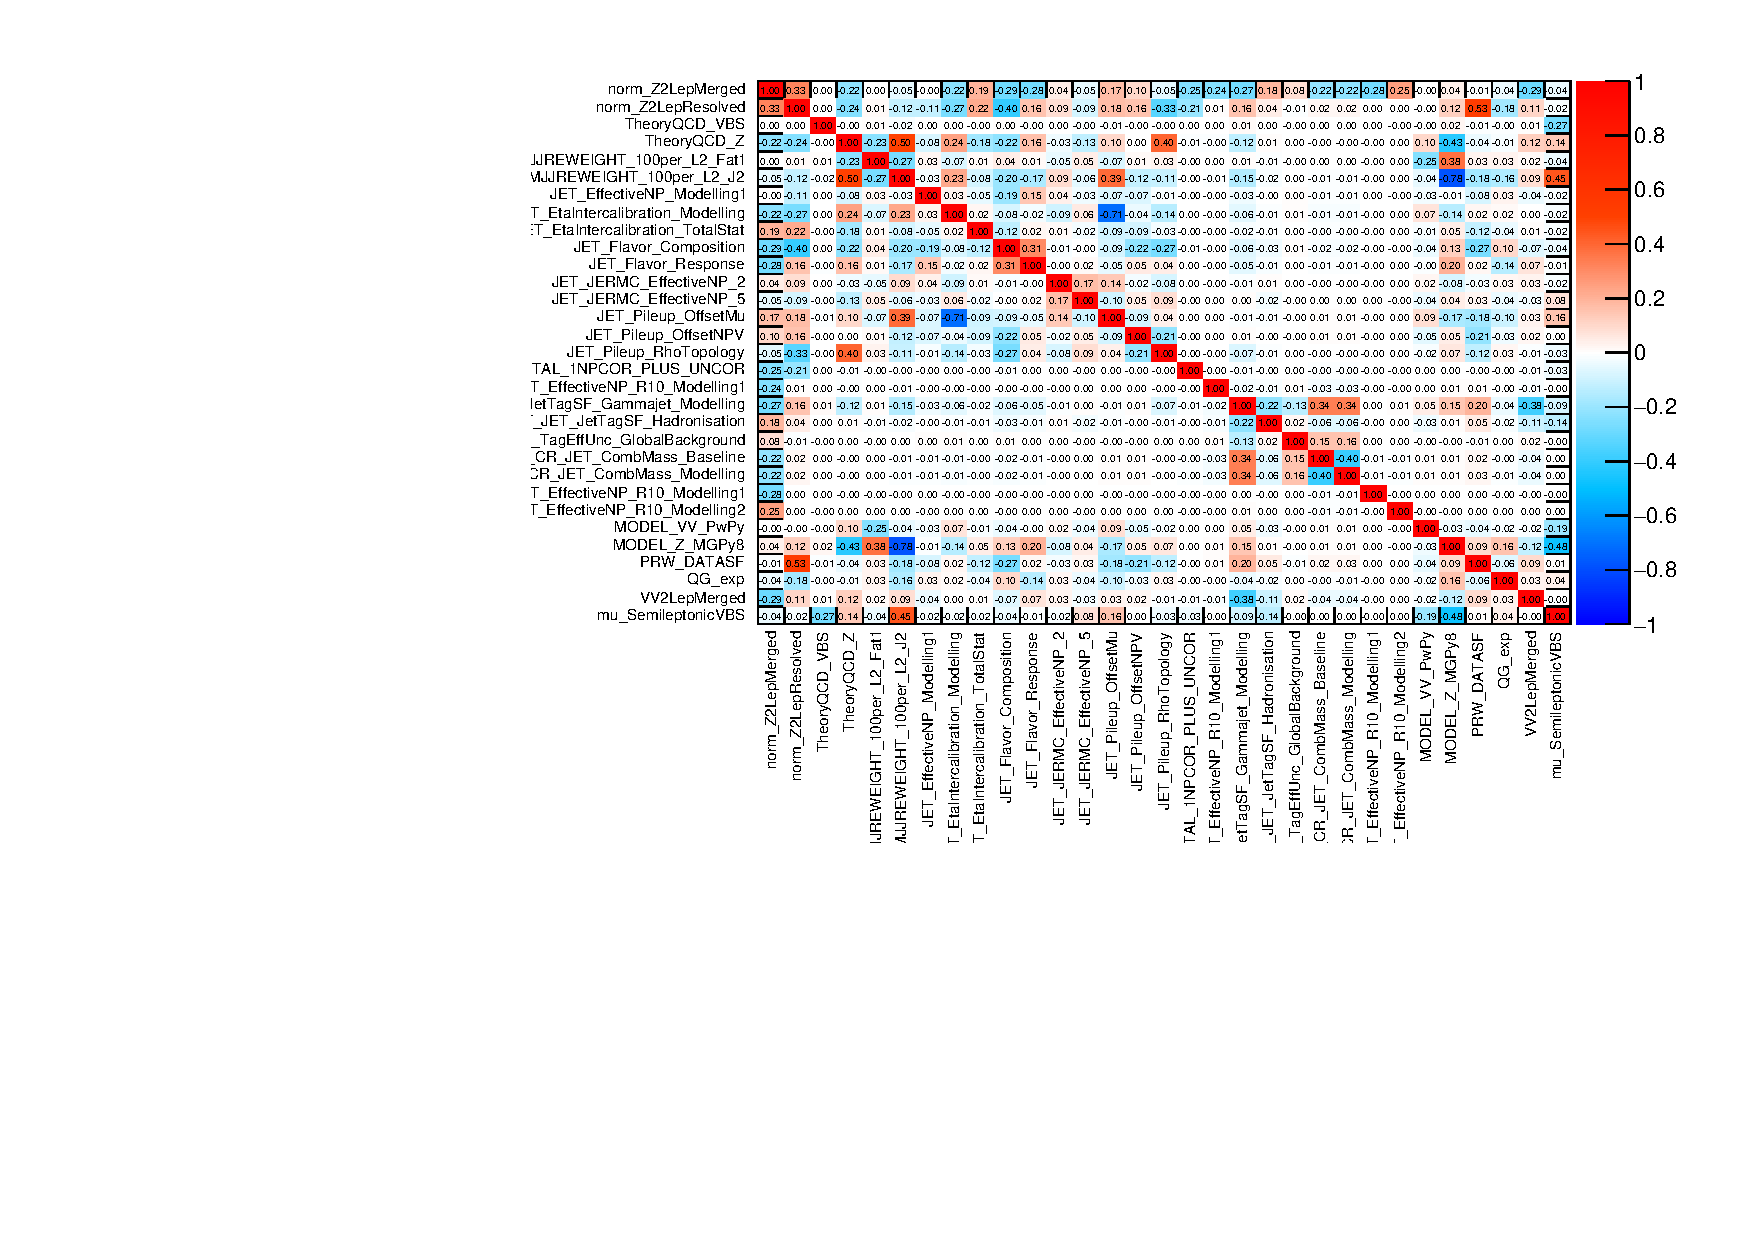
\includegraphics[width=\linewidth]{figures/2lep/FitResults/corr_HighCorrNoMCStat_AsimovAllbins.pdf}
        \caption{Correlations for unconditional fit ($\mu=1$) to asimov data in the full range, for the 2 lepton channel only.}
       \label{fig:fit_2lep_corr_all}
\end{figure}

\section{Rankings}
Ranking plots for all nuisance parameters without the bin-wise statistical uncertainties are shown in Figure~\ref{fig:fit_2lep_ranking_all}. The ranking plot shows the nuisance parameters which have large impact on the sensitivity. The ranking is derived by doing the scans of the likelihood function. First the nominal fit is performed to find the global maximum in the likelihood, and the corresponding $\hat{\mu}$. Then one nuisance parameter is fixed and scanned while all other parameters are fitted again. The scan as a function of one parameter stops once the logarithm of the likelihood decreases by 1/2 compared to the global maximum. This point corresponds to the 1~$\sigma$ uncertainty. The change of the signal strength, which is plotted as $\Delta\mu$ is evaluated here.
This scan is done with both direction of the NP and repeated for all NPs.
The top-two parameters are NPs relates to the Z+jet modeling issue and seen to be pulled in the pull plots. Varying these parameter by $1\sigma$ changes the signal strength by $\Delta \hat{\mu} \simeq 0.2$. The parameters which have strong impacts and highly-ranked are consistent with the parameters having strong correlations with the POI in the correlation plot, Figure~\ref{fig:fit_2lep_corr_all}.
\begin{figure}[ht]
      \centering
        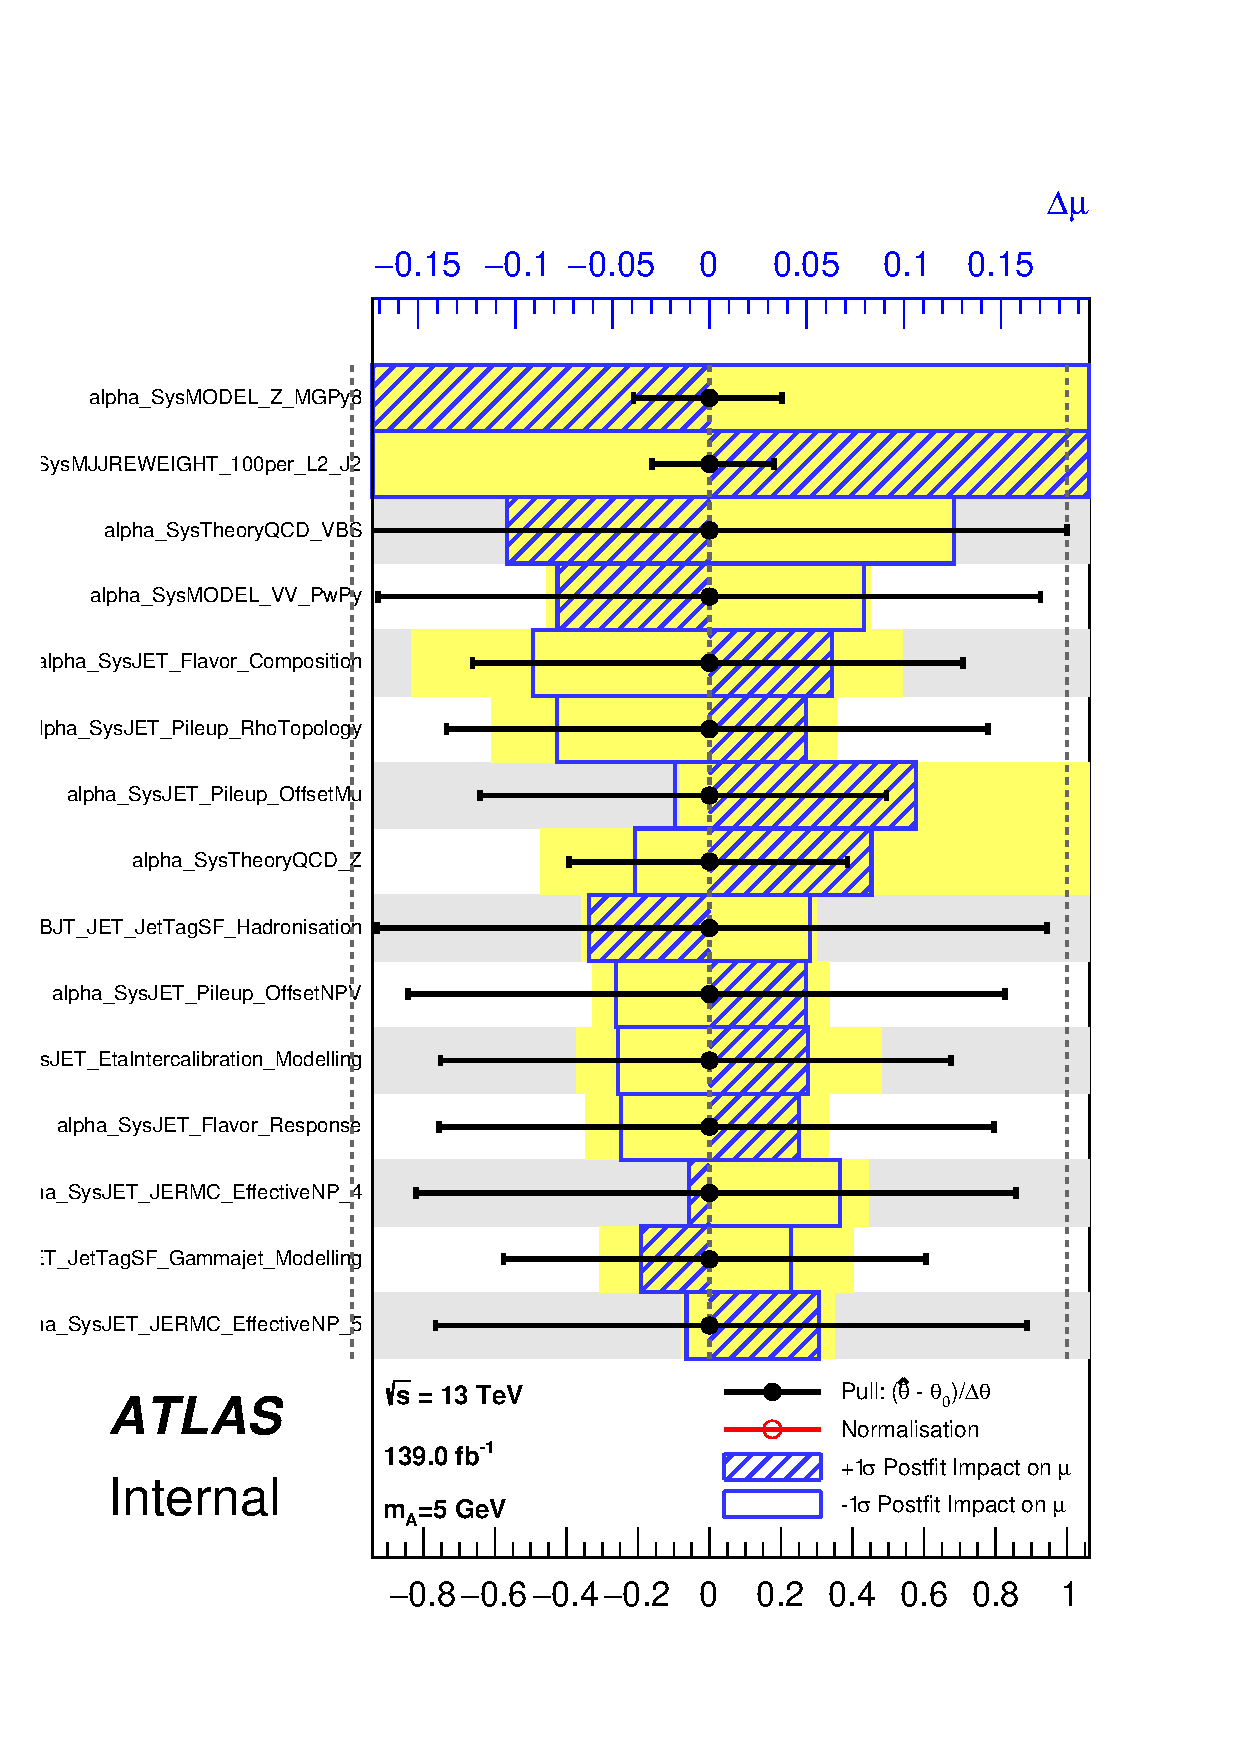
\includegraphics[width=0.8\textwidth]{figures/2lep/FitResults/pulls_mu_SemileptonicVBS_5_AsimovAllbins.pdf}
        \caption{Ranking plot for unconditional fit ($\mu=1$) to asimov data in the full range, for the 2 lepton channel only.}
       \label{fig:fit_2lep_ranking_all}
\end{figure}

\section{Results}
\subsection{Signal Strength}
The observed signal strength for the electroweak VVjj events in the fit for 2-lepton channel only is
\begin{equation}
***
%\hat{\mu}_{8 \mathrm{TeV}}=\sigma / \sigma_{\mathrm{SM}}=0.65_{-0.40}^{+0.43}
\end{equation}
